\section{Methodology}
\begin{figure}
    \centering
    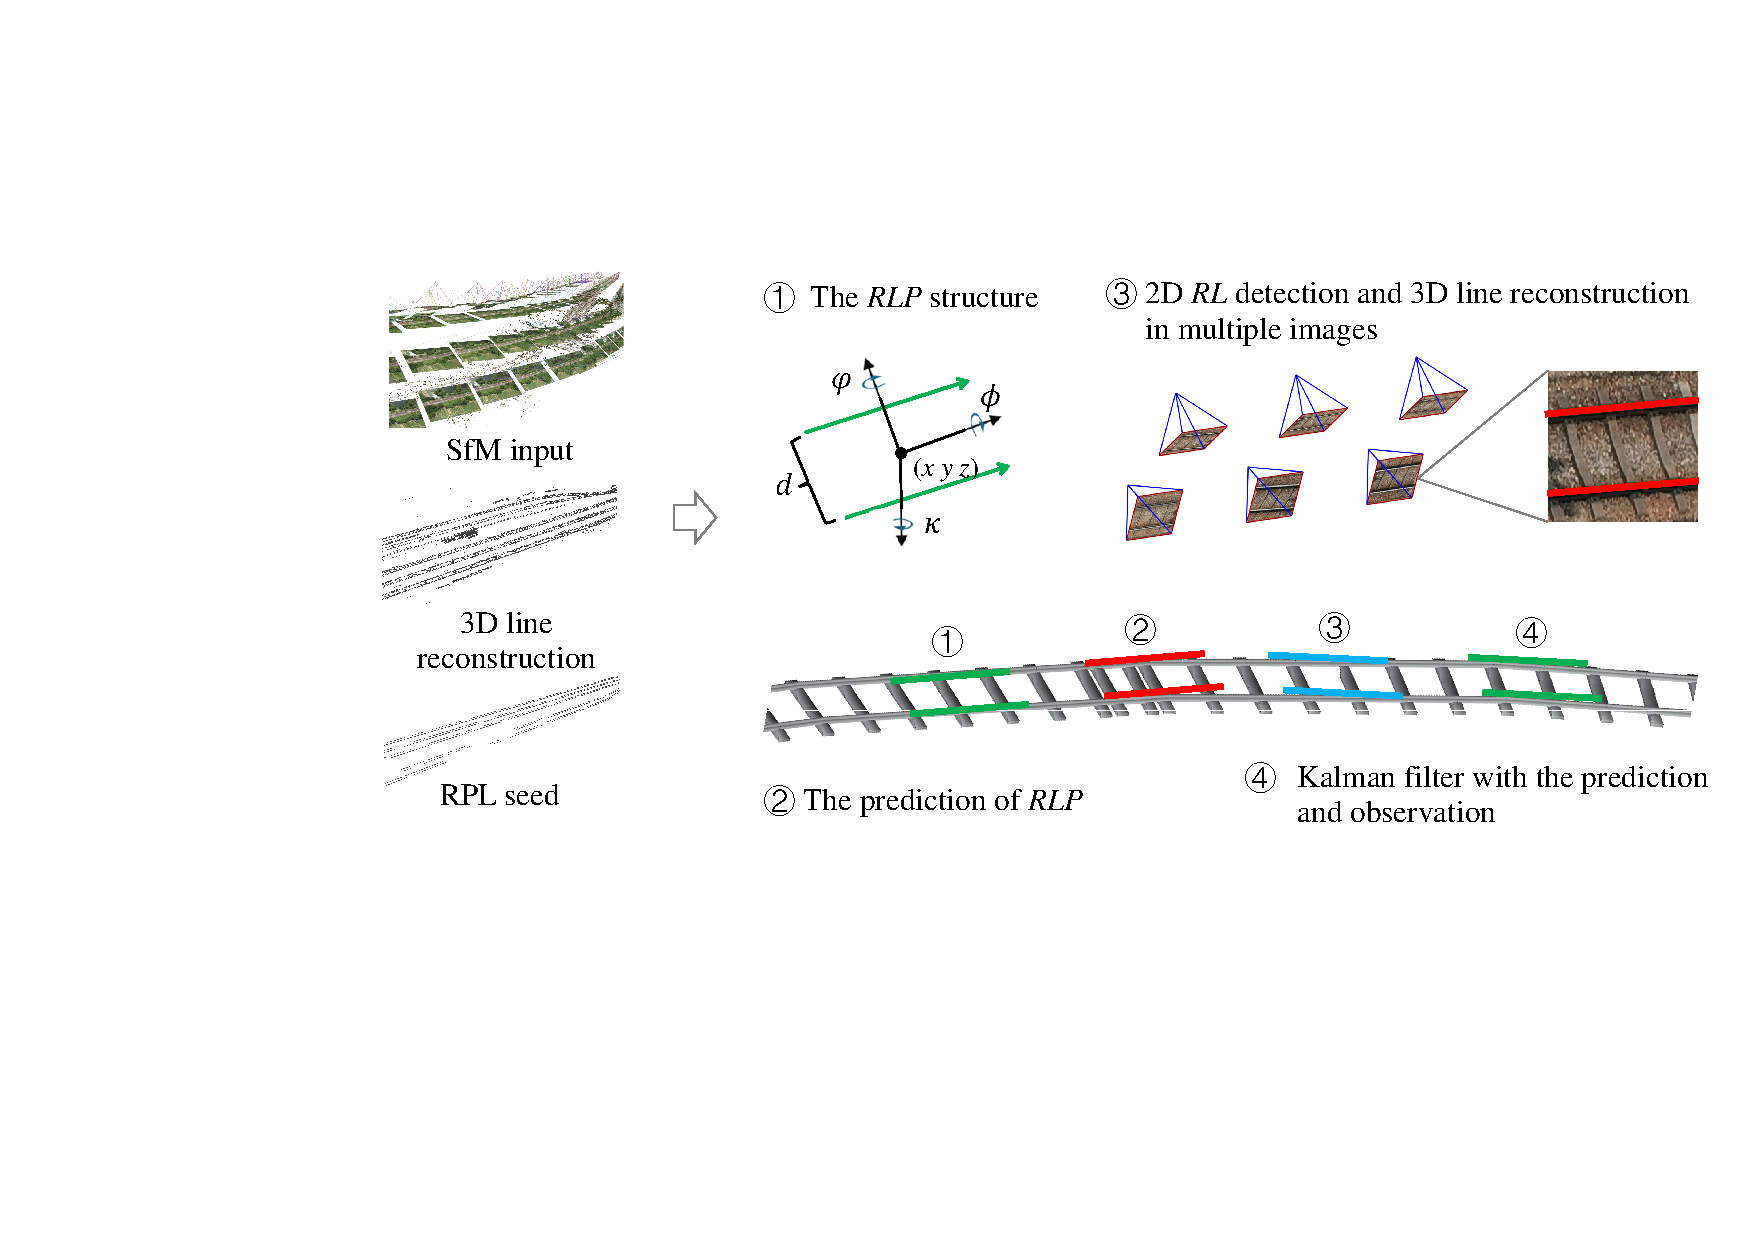
\includegraphics[width=0.9\textwidth]{images/overview.pdf}
    \caption{Visual alignment check in Kalman Filter.
    We project the estimation of \textit{RLP} in multiple images and extract the deep feature with pre-trained network.
    Then, 
    we check their cosine distance with the first $n/2$ cells in the queue,
    where $n$ is obtained by dividing the \textit{RLP} width by the step size $t$.}
    \label{fig_visualCheck}
\end{figure}
The flow of our methodology is presented in Figure 1.
We take aerial images of the railway area as input,
for which SfM and point clouds are used in advanced with existing software.
We first extract the image line and convert it to a space line with the locally optimal plane of the point cloud.
Then,
we cluster the single 3D line to RT candidates with the frame work derived from DBSCAN,  
during which the texture information of multiple images extracted from ResNet is used as one of the inlier distance.
Having obtained the RT cluster, 
we then trace and reconstruct the vector-based RT in the Kalman framwork,
which fully exploits the RT structure and the multi-view geometries to resolve the uncertainty caused by initial image line segment extraction and the point cloud error.
The railway-track pair is the start seed of our Kalman method.
We first convert image lines to 3D lines with the local optimal plane of the point cloud.
Then,
we cluster the single 3D line to RT pairs with DBSCAN frame work,  
during which the deep feature of multiple images is used as the inlier distance.
Since the 

\subsection{Initial seed generation}

We group two 3D lines as a RT pair based on their angle $\theta_{i,j}$,
overlap $o_{i,j}$,
and projection distance $d_{i,j}$:
\begin{equation}
   \left\{ RT= \left(L_i, L_j\right) \mid \theta_{i,j} < t_\theta, o_{i,j} > t_o, d_{i,j} \in I  \right\},
    \label{eq_geometrycons}
\end{equation}
$\theta_{i,j}$ and $o_{i,j}$are easy to choose,
e.g.,
$5^\circ$ and 60\%,
because the RT pair is parallel and highly overlapped;
while the interval $I$ needs the rough width $\omega$ between the two RT,
which can be acquired from construction standards or point clouds.
We recommend setting $I=\left[2/3\omega,4/3\omega\right]$ that uses one-third of $\omega$ as the margin of error.
Because a 3D line may satisfy \cref{eq_geometrycons} with many others,
the greedy algorithm is used to assign the candidate pair,
which uses the sum of the overlap rate as the maximum score.
We sort the RT based on their scores of the geometry alignment and select the top 10\% RT and use contextual information to further validate the RT pair.
In detail,
if the RT's central line is within $1^\circ$ and $t$ projection distance with another RT,
its score is increased by $\mathcal{N}\left(\mu, \left(t/3\right)^2\right)$.

\begin{figure}[h]
    \centering
    \includegraphics[width=0.9\textwidth]{images/initialSeed.pdf}
    \caption{Visual alignment check in Kalman Filter.
    We project the estimation of \textit{RLP} in multiple images and extract the deep feature with pre-trained network.
    Then, 
    we check their cosine distance with the first $n/2$ cells in the queue,
    where $n$ is obtained by dividing the \textit{RLP} width by the step size $t$.}
    \label{fig_visualCheck}
\end{figure}

Considering the texture along the \textit{RLP} should be roughly the same, 
as illustrated in \cref{fig_visualCheck},
we use the global average pooling layer in ResNet101 as the basic feature,
which has been trained on massive amounts of data and can capture texture patterns for classification in the absence of labels,
to confirm the initial seed and check for termination.
Denoting $\mathbf f \in R^n$ as the \textit{RLP} feature,
we acquire the set of features $\left\{\mathbf f_i\right\}_{i=1}^m$ from the $m$ support images.
To reduce the ambiguity of the deep feature caused by scale and rotation,
the image block is transformed to ensure that the center line of \textit{RLP} passes through the image center horizontally and the width of \textit{RLP} is half of the image.
After extraction of RT features, 
we use DBSCAN to group them with the cosine distance,
and retain the group with the highest number as the seeds of RT.



\subsection{Railway track with Kalman filter}
As shown in, 
we use two points and directions to represent the state of the local \textit{RLP}.
Denote the point and direction as
$\mathbf p=\left(x,y,z\right)$ and $\mathbf d=\left(dx,dy,dz\right)$,
respectively.
The vector to be estimated for the \textit{RLP} is
\begin{equation}
\mathbf x = \begin{bmatrix}
    \mathbf p_1 & \mathbf p_2 & \mathbf d_1  & \mathbf d_2 
\end{bmatrix}^ \top \in R^{12}.
\label{eq_prediction3} 
\end{equation}
The prediction of $\mathbf x$ is controlled by a scalar $t$:
\begin{equation}
        \mathbf{x}^{pre}= 
        \mathrm F \mathbf x^{{\mbox -}}, \in R^{12}, \quad  
        \mathrm F=\operatorname{diag}\left(t \! \cdot \! \mathrm I_{6\times6} , \mathrm I_{6\times6}\right) \in R^{12\times 12},
        \label {eq_statetransition}
\end{equation}
where the superscript $^{\mbox -}$ marks the previous state.
For each prediction $\mathbf{x}^{pre}$,
There is an actual observation $\mathbf{x}^{obs}$ arising from line reconstruction in multiple images~(\cref*{sec_linereconstruction}).
The \textit{RLP} has fixed geometry patterns,
i.e.,
$\mathbf d_1$ and $\mathbf d_2$ should be as close as possible,
and the distance change between $\mathbf p_1$ and $\mathbf p_2$ is as small as possible.
We achieve these two constraints by extending the observation vector:
\begin{equation}
\mathbf{z}^{obs} = \begin{bmatrix}
    \mathbf{x}^{obs} & \mathbf p_1^{\mbox -} - \mathbf p_{2}^{\mbox -} & \mathbf 0_{1\times3}
\end{bmatrix}^ \top \in R^{18}.
\label {eq_observationvector}
\end{equation}
Correspondingly,
the observation matrix that translate $\mathbf{x}^{pre}$ to the observation form is
\begin{equation}
        \mathbf{z}^{pre}= 
        \mathrm H \mathbf x^{pre}, \quad  
        \mathrm H=
        \begin{bmatrix}
            \multicolumn{4}{c}{\mathrm{I}_{12 \times 12}} \\
            \mathrm{I}_{3 \times 3} & -\mathrm{I}_{3 \times 3} & \mathbf{0}_{3 \times 3} & \mathbf{0}_{3 \times 3} \\
            \mathbf{0}_{3 \times 3} & \mathbf{0}_{3 \times 3} & \mathrm{I}_{3 \times 3} & -\mathrm{I}_{3 \times 3}
        \end{bmatrix} \in R^{18 \times 12}.
        \label {eq_observationmatrix }
\end{equation}
Then,
as shown in \cref{fig_kalmanflow},
we use the general discrete Kalman filter to update the state.
\begin{figure} [h]
    \centering
    \resizebox{0.9\textwidth}{!}{%
    \begin{circuitikz}
    \tikzstyle{every node}=[font=\normalsize]
    
    % 右侧矩形 (b)
    \draw [rounded corners=5pt]  (0,23.5) rectangle  
    node {\large
    \begin{minipage}{6cm}
    (b)~$\mathbf{z}^{obs}$ (\cref{eq_observationvector}) calculation via
    3D line reconstruction.  
    \end{minipage}
    } (6.25,21.5);
    
    % 右侧矩形 (a)
    \draw [rounded corners=5pt] (0,20.5) rectangle  
    node {\large
    \begin{minipage}{6cm}
    (a)~$\mathbf{x}^{pre}$ prediction  with \cref{eq_statetransition}
    and error covariance prediction via 
    \vspace{-0.5em}
    \begin{equation}
    \mathrm P^{pred}= \mathrm F \hat{\mathrm {P}}\mathrm F^{\top}+\mathrm Q
    \label{eq_xprediction}
    \end{equation}
    \end{minipage}
    }  (6.25,18.5);
    
    % 右侧大矩形,右移 0.5 单位
    \draw  [rounded corners=5pt] (8.0,23.5) rectangle  
    node {
        \large
    \begin{minipage}{7cm}
    (c)~Kalman gain update :
    \begin{equation}
    \mathrm K= \mathrm P \mathrm H^{\top}
    \left(\mathrm H \mathrm P \mathrm H^{\top}+\mathrm R\right)^{-1}
    \label{eq_kalmangain}
    \end{equation}
    (d)~estimation update:
    \begin{equation}
    \mathbf{\hat{x}}= \mathbf x^{pre} + \mathrm K \left(\mathbf{z}^{pre}- \mathbf{z}^{obs}\right)
    \end{equation}
    (e)~error covariance update:
    \begin{equation}
    \hat{\mathrm {P}} = \left( \mathrm{I} - \mathrm{K} \mathrm{H} \right) \mathrm{P}^{pre}
    \end{equation}
     \end{minipage}
    } (15.5,18.5);
    
    % 拉长的右侧箭头
    \draw [->, >=Stealth] (6.25,22.5) -- (8.0,22.5); % 拉长到 8.0
    \draw [->, >=Stealth] (8.0,19.5) -- (6.25,19.5); % 拉长到 8.0

    % 左侧矩形 Initial estimate,左移 0.5 单位
    \draw [fill=gray!10,rounded corners=5pt] (-7.7,20.5) rectangle  
    node {\large
    \begin{minipage}{5cm}
    Initial estimation of $\mathbf {\hat{x}}$~(\cref{sec_seedgeneration}) and the initial covariance error $\hat{\mathrm {P}}=\mathrm{I}_{12\times 12}$
    \end{minipage}
    } (-1.72,18.5);
    
    % 左侧矩形 Check for termination,左移 0.5 单位 []
    \draw [fill=gray!10,rounded corners=5pt] (-7.7,23.5) rectangle  
    node {\large
    \hspace{0.4em} 
    \begin{minipage}{5.5cm}
        \raggedright % 使标题顶格
        Check for termination:
        \vspace{-1em}
        \begin{itemize}
            \setlength{\itemsep}{0pt} 
            \setlength{\parskip}{0pt} 
            \setlength{\parsep}{0pt}
            \setlength{\leftskip}{0pt} % 保持item缩进
            \item non-convergence of reconstruction~(\cref{sec_linereconstruction})
            \item visual inconsistency
            \item positional overlap 
        \end{itemize}
    \end{minipage}
    } (-1.72,21);

    % 拉长的左侧箭头
    \draw [->, >=Stealth] (-1.72,19.5) -- (0,19.5); % 左侧箭头延长到 -1.72
    \draw [<-, >=Stealth] (-1.72,22.5) -- (0,22.5); % 左侧箭头延长到 -1.72
    
    \end{circuitikz}
    }%
    \caption{The flow of kalman filter for the \textit{RLP} estimation.$\mathrm{Q}$ in \cref{eq_xprediction} and $\mathrm{R}$ in \cref{eq_kalmangain} represents the covariance matrix of observation noise and process noise,respectively.}
    \label{fig_kalmanflow}
\end{figure}

\subsection{Accurate railway line measurement}
\label{sec_linereconstruction}
For a 3D line in $\mathbf{x}^{pre}$~(\cref{eq_statetransition}),
we convert it into image with camera matrix and obtain the 2D line segment
$\mathbf{l}^{pre}=\begin{bmatrix} x_c,y_c,\theta \end{bmatrix}$;
then we search around $\mathbf{l}^{pre}$ for the observation $\mathbf{l}^{obs}$,
which should have the maximum gradient response:
\begin{equation}
 \mathcal{L} = \sum_{i=1}^{N} \lambda_i \cdot \|G_x \left(x_i, y_i \right),G_y\left(x_i, y_i\right) \|^2, 
\label{eq_GDobjfunction}
\end{equation}
where $G_x$ and $G_y$ is the gradient magnitude in two dimensions;
the sample point is calculated by
\begin{equation}
\begin{bmatrix}
x_i \\
y_i
\end{bmatrix}
=
\begin{bmatrix}
x_c \\
y_c
\end{bmatrix}
+
\begin{bmatrix}
\cos\theta & -\sin\theta \\
\sin\theta & \cos\theta
\end{bmatrix}
\begin{bmatrix}
h_i \\
p_i
\end{bmatrix},
\label{eq_samplepoints}
\end{equation}
where $h_i$ and $ p_i$ is the parallel and horizontal distance of $\mathbf{l}^{obs}$,
respectively.
Because the \textit{RL} has a width that is different at different positions in different images,
we use $\lambda_i$ to weight the gradients:
\begin{equation}
\lambda_i= 1 - \frac{1}{1 + e^{10\left(w_1-p_i \right)}} + \frac{1}{1 + e^{10\left(w_2-p_i\right)}}
\end{equation}
where $w_1$ and $w_2$ are the distance calculated from the the prior width of \textit{RL}.
We use the gradient ascend,
\begin{equation}
\mathbf{l}^{obs}_{i}=\mathbf{l}^{obs}_{i-1}-\alpha \Delta \mathcal{L},
\label{eq_gditerative}
\end{equation}
to find $\mathbf{l}^{obs}$ with \cref{eq_GDobjfunction},
where \( \alpha \) is the learning rate.
\( \Delta \mathcal{L} \) is the gradient from \cref{eq_GDobjfunction} and \cref{eq_samplepoints}:
\begin{equation}
\Delta \mathcal{L} = - \sum_{i=1}^{N} \lambda_i \mathbf{J}_i
\begin{bmatrix}
G_x(x_i, y_i) &
G_y(x_i, y_i)
\end{bmatrix}^{\top},
\end{equation}
where $\mathbf{J}_i$ is the Jacobian matrix
\begin{equation}
\mathbf{J}_i=
\begin{bmatrix}
\partial x_i / \partial x_c & \partial x_i / \partial y_c & \partial x_i / \partial \theta \\
\partial y_i / \partial x_c & \partial y_i / \partial y_c & \partial y_i / \partial \theta
\end{bmatrix}^{\top}
\end{equation}

\cref{eq_gditerative} takes $\mathbf{l}^{pre}$ as input and iterates until the parameters converge, i.e., when the change in the parameters is smaller than a predefined threshold.
After the measurement in multiple images, 
we obtain a set of image lines and the accurate 3D line is reconstructed with the method in (ref).

\subsection{Initial seed and termination with deep features}


\textbf{Check for termination.} We save the set that has passed texture validation in a queue and use the first half of the elements in the queue to validate the new $\left\{\mathbf f^\prime\right\}_{i=1}^{m1}$:
\begin{equation}
\sum_{i=1}^{m_1} \mathbb{I} \left( \exists j \in \left[ m_2 \right], \, \cos \left( \mathbf{f}_i, \mathbf f^{\prime}_j \right) > \theta \right) \geq \frac{m_1}{2}
\label{eq_featureValidation}
\end{equation}
where $m2$ is the total number of $\mathbf f$ in the first half of the feature set in the queue;
$\mathbb{I}$ represents an indicator function which takes the value of 1 when a certain condition is true and 0 otherwise.
If $\left\{\mathbf f^\prime\right\}_{i=1}^{m1}$ satisfy \cref{eq_featureValidation},
it is pushed to the queue, 
and then the queue is dequeued if its cell passed $cal$.

\begin{figure}
    \centering
    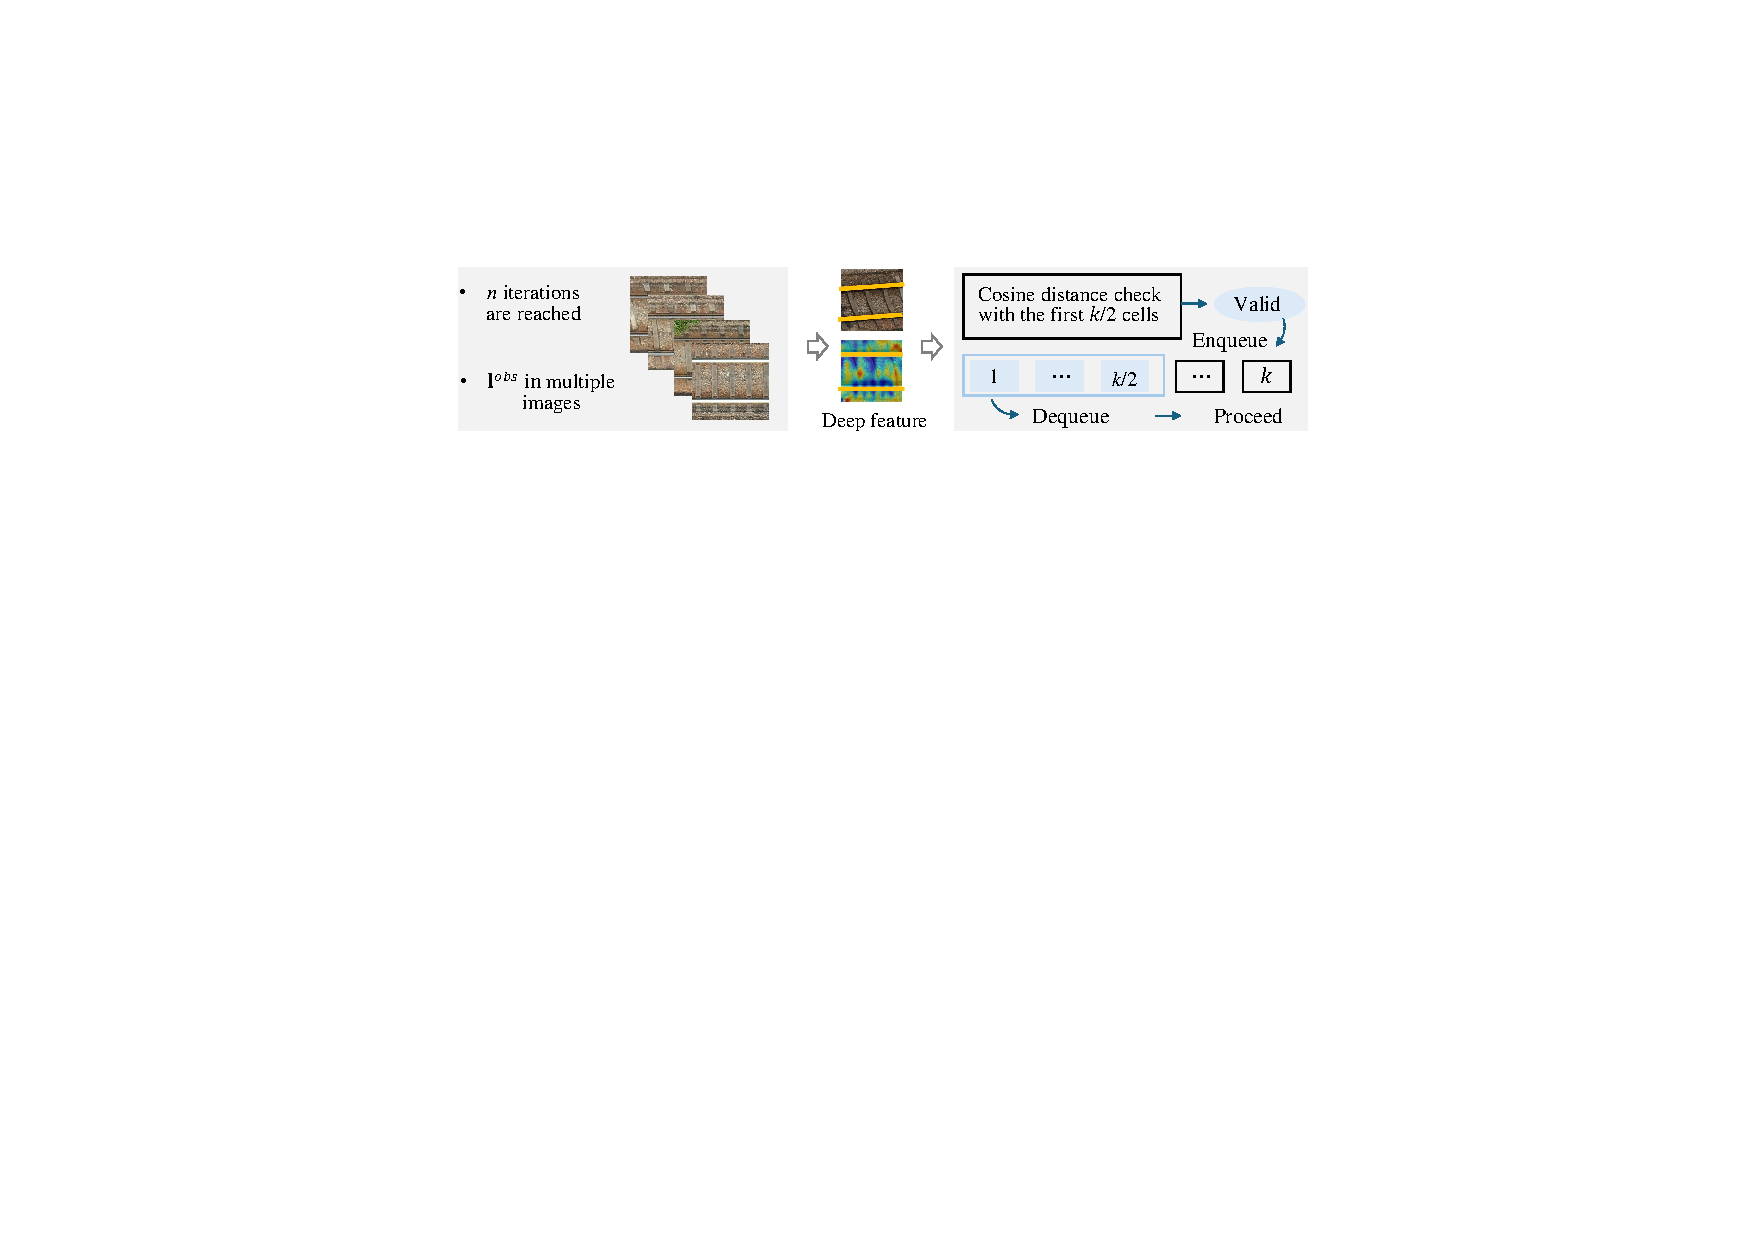
\includegraphics[width=0.9\textwidth]{images/visualCheck.pdf}
    \caption{Visual alignment check in Kalman Filter.
    We project the estimation of \textit{RLP} in multiple images and extract the deep feature with pre-trained network.
    Then, 
    we check their cosine distance with the first $n/2$ cells in the queue,
    where $n$ is obtained by dividing the \textit{RLP} width by the step size $t$.}
    \label{fig_visualCheck}
\end{figure}







